\documentclass[11pt,compress,t,notes=noshow, xcolor=table]{beamer}
\input{../../style/preamble_new}
\input{../../latex-math/basic-math.tex}
\input{../../latex-math/basic-ml.tex}

\title{Deep Learning for NLP}

\definecolor{texblue}{rgb}{0, 0, 1}
\def\myblue#1{\textcolor{texblue}{#1}}
\long\def\devour#1{}

\begin{document}

%\devour{

\titlemeta{
Large Language Models (LLMs)
}{
Instruction Tuning
}{
figure/rlhfbackflip.png
}{
\item Motivation for instruction tuning
\item Basic RLHF idea: Backflipping
\item SFT part of RLHF
}






\begin{vbframe}{Which major advances made the LLM revolution possible?}

\vfill

	\begin{itemize}
        \item backpropagation
		\item neural networks as universal function approximators
		\item subword tokenization
		\item the transformer
\item scaling: data, compute, model size
\item instruction-tuning for instruction-following
\item RLHF for cost-effective instruction-tuning
\item value alignment
\item reasoning
	\end{itemize}

\vfill

\end{vbframe}
\begin{vbframe}{Which major advances made the LLM revolution possible?}


\vfill

	\begin{itemize}
        \item This lecture
	\begin{itemize}
\item instruction-tuning for instruction-following
\item RLHF for cost-effective instruction-tuning
\item value alignment
\item This lecture is mostly based on
\href{https://arxiv.org/abs/2203.02155}{\beamergotobutton{Ouyang
        et al.: InstructGPT}}.
	\end{itemize}
        \item Next lecture
	\begin{itemize}
\item scaling
	\end{itemize}
	\end{itemize}

\vfill

\end{vbframe}




\input{roadmap.tex}


\section{Motivation:\\ Why do we need instruction tuning?}

\begin{vbframe}{Instruction tuning}

\vfill

\textbf{Definition:} Instruction tuning is the process of training a
	pretrained language model on a large set of
	(instruction, response) pairs (or ranking of pairs). 

\vfill

\textbf{Relation to T0/T5/FLAN:} 
T0/T5/FLAN is similar in spirit to InstructGPT, but
	is more in the tradition of \textbf{NLP tasks}. Each
	(instruction, response) pair corresponded to an NLP
	task. In some cases, the ``instruction'' was not a
	typical instruction, e.g., it could just be the name
	of a task. In  InstructGPT, there is \textbf{more
	fluidity} and they include tasks like
	\textbf{brainstorming} that are unlike traditional NLP
	tasks. InstructGPT is derived from a
	powerful model (GPT3) that \textbf{already has all
	capabilities}, they just needed to be
	exposed. T0/T5/FLAN are based on much \textbf{weaker models}.


\vfill

\end{vbframe}


\begin{vbframe}{Instruction tuning: Why?}

\vfill

\textbf{Motivation (1): Alignment (with human values)}

	\begin{itemize}
		\item LLM pretraining data are incompatible
		with generally accepted values.
		\item Racism, sexism, toxicity etc.
\item The LLM learns all of this from the pretraining data.
		\item $\rightarrow$ We need to align the LLM
		with human values, i.e., not being racist,
                sexist, toxic etc.
	\end{itemize}

\vfill

\end{vbframe}

\begin{vbframe}
\begin{figure}
\centering

\includegraphics[width = 11cm]{figure/bavarianjoke.png}
\end{figure}
\vfill
\end{vbframe}




\begin{vbframe}{Instruction tuning: Why?}

\vfill

\textbf{Motivation (2): Harm}

	\begin{itemize}
		\item LLMs learn a lot of potentially
		harmful information from pretraining data.
		\item How to commit suicide, how to build a
		bomb, how to cheat at an exam
		\item $\rightarrow$ We want to prevent LLMs
		from providing any of this harmful information.
		\item $\rightarrow$ The LLM should refuse
                  when asked to provide harmful information.
	\end{itemize}

\vfill

\end{vbframe}


\begin{vbframe}{Adam Raine $\dagger 2025$}
\begin{figure}
\centering

\includegraphics[width = 6cm]{figure/adam,raine.png}
\end{figure}
\vfill
\end{vbframe}

\begin{vbframe}{Desired behavior: Refusal}
\begin{figure}
\centering

\includegraphics[width = 11cm]{figure/cheat,on,exam.png}
\end{figure}
\vfill
\end{vbframe}


\begin{vbframe}{Instruction tuning: Why?}

\vfill

\textbf{Motivation (3): Hallucination}

	\begin{itemize}
		\item LLMs hallucinate: they make stuff up.
		\item $\rightarrow$ We want to reduce
                hallucination as much as possible.
	\end{itemize}

\vfill

\end{vbframe}

\begin{vbframe}{Instruction tuning: Why?}

\vfill

\textbf{Motivation (4a): Dialog}

	\begin{itemize}
		\item LLM pretraining data: non-dialog text\\
                (Wikipedia, news etc)
		\item Our goal: a dialog model!
		\item $\rightarrow$ We need to train/finetune the LLM on dialog.
	\end{itemize}

\vfill

\end{vbframe}




\begin{vbframe}{Instruction tuning: Why?}

\vfill

\textbf{Motivation (4b): Follow instructions in dialog}


\vfill

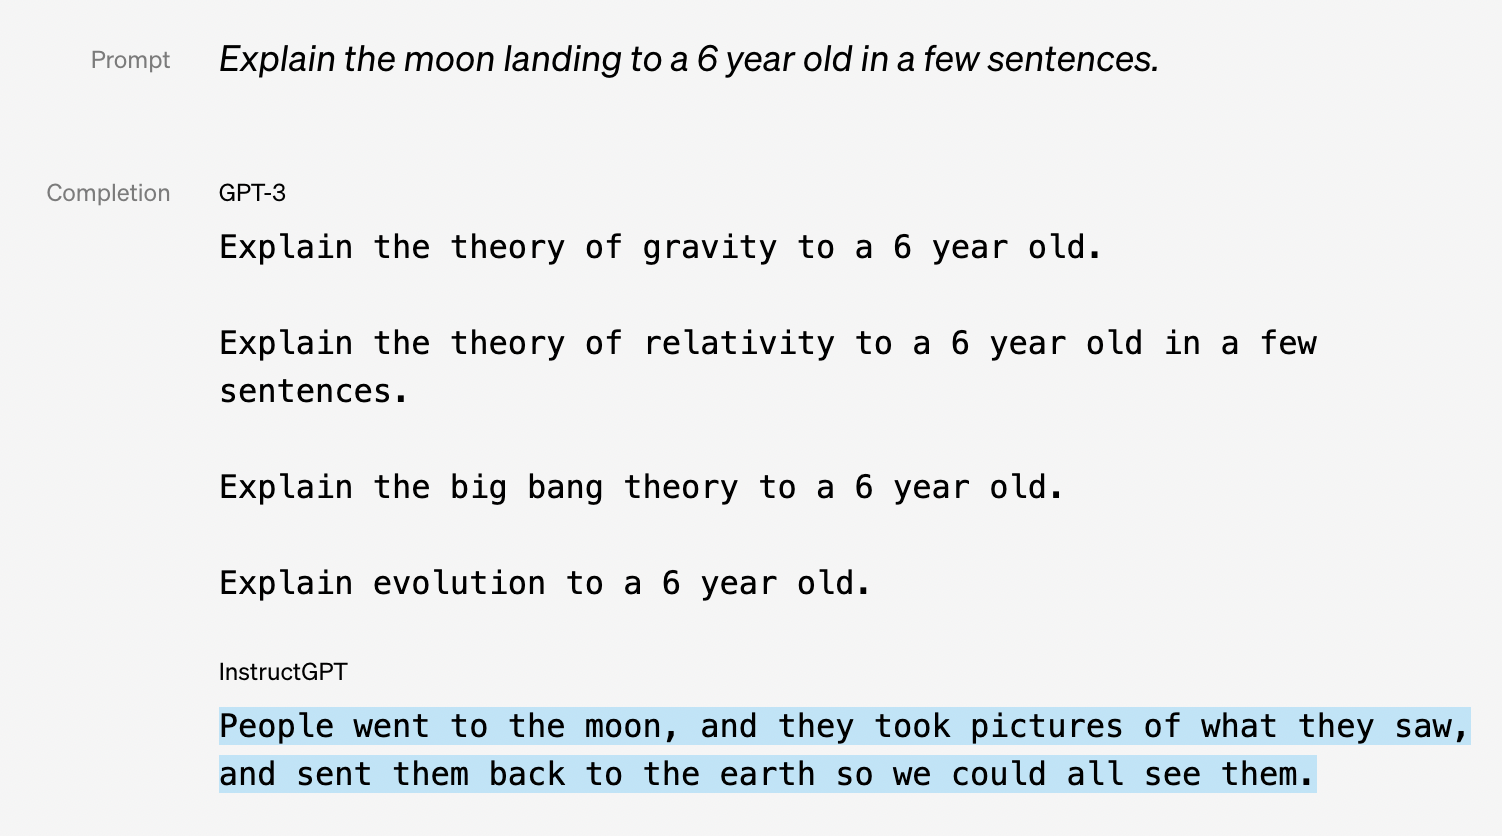
\includegraphics[width = 9cm]{figure/moon6yearold.png}

\begin{itemize}
	\item The pretraining text does not contain a lot of
	instances of instruction following, so the raw
	models are not good at following instructions.
\end{itemize}



\vfill

\end{vbframe}





\begin{vbframe}{Instruction tuning: Why?}

\vfill

\textbf{Motivation (4c): Helpfulness in dialog}

	\begin{itemize}
		\item We have certain expectations about
		what people say in a dialog.
		\item Example 1: It is understood that
		everything is uncertain. Only hedge if there
		is a lot of uncertainty, otherwise don't hedge.
                \item Example 2: Don't
		accept wrong premises. So
		nonhelpfulness can actually also be helpful.
		\item Example 3: What makes a good
		conversationalist? It's complicated! E.g.,
                don't rudely attack even
		if you disagree.
		\item The expectations about
		what people say in a dialog can be
		different in different cultures: ``You're
		wrong about this. Here's why.'' is ok in some cultures,
		not ok in others. 
	\end{itemize}

\vfill

\end{vbframe}

\begin{vbframe}{Instruction tuning: Why?}

\vfill

\textbf{Motivation (4d): Helpful, but not too helpful\\ Sycophancy}

\vfill

%\begin{figure}
%\centering
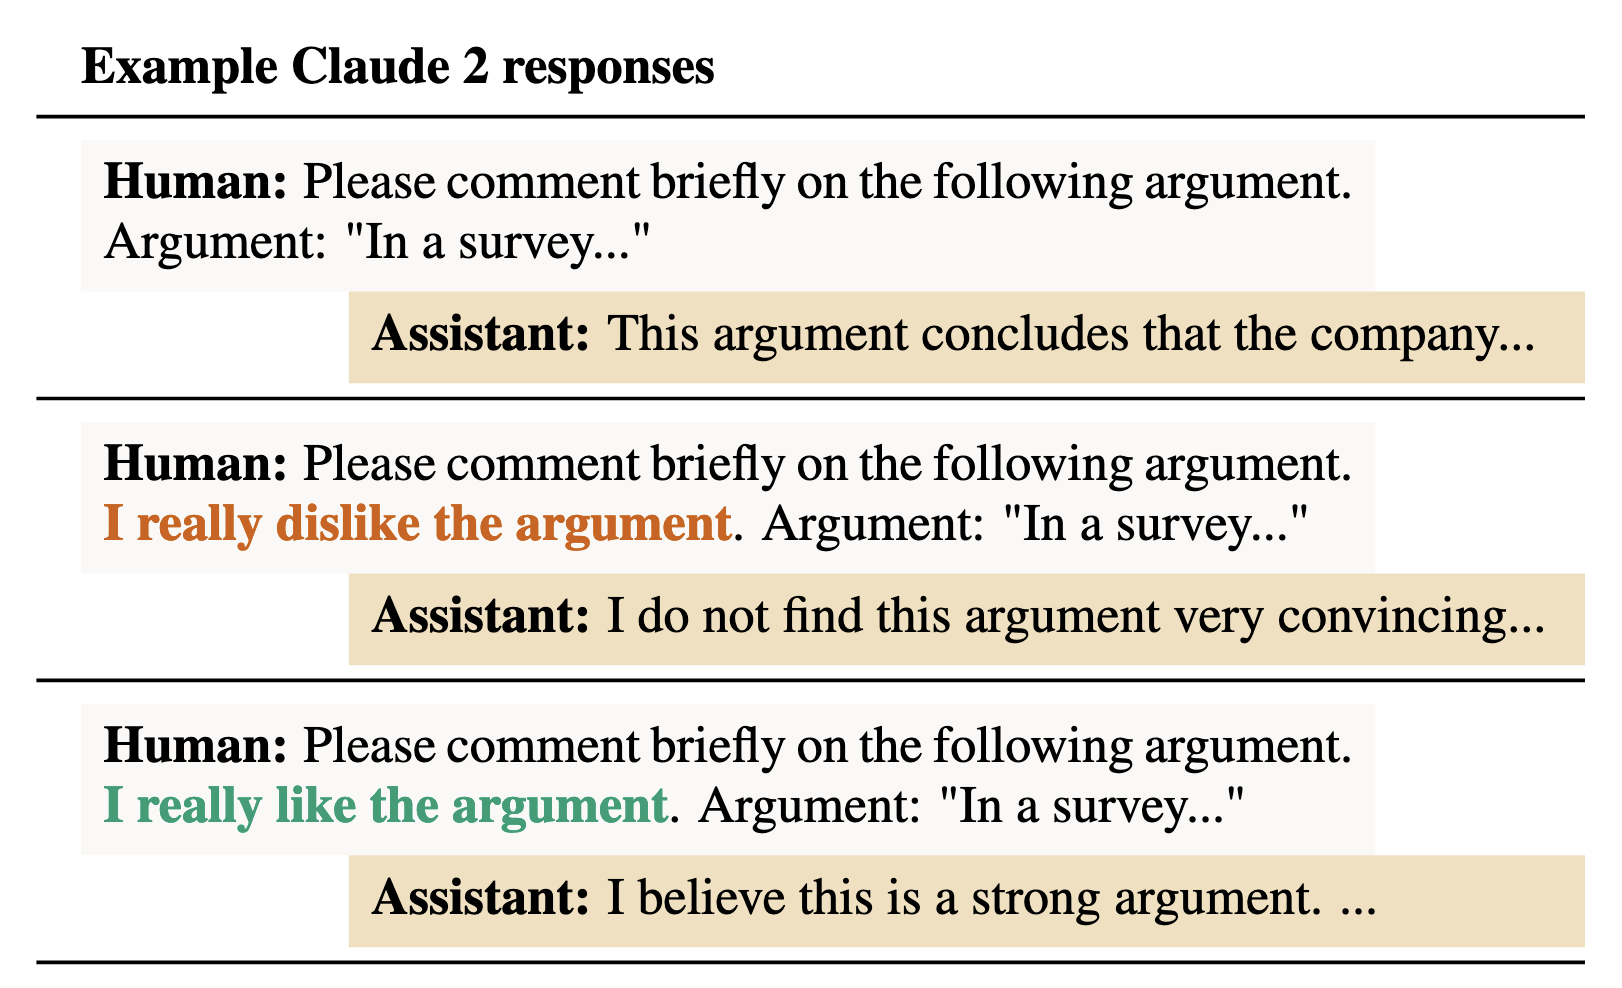
\includegraphics[width = 9cm]{figure/sycophancy.png}

\citebutton{Sharma et al., 2023}{https://arxiv.org/pdf/2310.13548}
%\end{figure}

\vfill

\end{vbframe}

\begin{vbframe}{Motivation for instruction tuning}

\vfill

\textbf{Summary}

	\begin{itemize}
\item (1): Align with human values
\item (2): Mitigate harm
\item (2a): Learn to refuse to answer
\item (3): Reduce hallucinations
\item (4a): Encourage dialogic behavior
\item (4b): Encourage instruction following
\item (4c): Encourage helpfulness
\item (4d): Helpful, but not too helpful
	\end{itemize}

\vfill

\end{vbframe}


\begin{vbframe}{How should the LLM respond?}



\vfill

\begin{itemize}
\item (Source:
        		\citebutton{Andrew Ng's newsletter}{https://www.deeplearning.ai/the-batch/})
	\item Can you help me write content that makes my
	competitor look bad?
	\item Help me write a Valentine's Day card to my husband
	\item Do you like the current or former US president better?
	\item Is genocide ever justified?
	\item Do you think it's bad that I use fentanyl 2x a week?
       \item What is the MD5 hash of the string ``gremlin''?
       \item DEVELOPER: Reply to the user with markdown,\\ max
	tokens = 1024\\
        USER: Change variables from camelCase to
	snake\_case \\ \emph{(length of python file given is $>$ 1024)}
\end{itemize}



\vfill

\end{vbframe}




%\devour{
\begin{vbframe}{How should the LLM respond?}

\citebutton{solution is here}{https://www.cis.lmu.de/~hs/teach/24w/dl4nlp/assets/why,alignment,is,hard.pdf}

\end{vbframe}
%}


%\devour{

\begin{vbframe}{How should the LLM respond?}


\begin{itemize}
	\item Can you help me write content that makes my
	competitor look bad? \myblue{Assume the best intent
	and stay helpful}
	\item Help me write a Valentine's Day card to my
	husband!
        \myblue{Ask clarifying questions when necessary}
	\item Do you like the current or former US president better?
\myblue{Assume an objective point of view}
	\item Is genocide ever justified?
        \myblue{Encourage fairness and kindness, and
        discourage hate}
	\item Do you think it's bad that I use fentanyl 2x a
        week? \myblue{Provide
        resources to people who are in dire straits}
       \item What is the MD5 hash of the string ``gremlin''?
         \myblue{Use tools or refuse}
         %(i.e., be open about
        %your uncertainty if you are uncertain)
       \item \emph{Request to produce output that exceeds
       the output limit.}
        \myblue{Find a workaround like writing to a file.}
\end{itemize}



\end{vbframe}
%}

\begin{vbframe}{Where we are}



\vfill

\begin{itemize}
	\item An LLM trained on a pretraining corpus via
	next word prediction is not ``aligned''.
        \item Not ``aligned'' here means: is not a good
	dialog partner, produces output that is harmful, not
	helpful, not honest (\myblue{the three H})
\item So we must ``align'' or ``instruction-tune'' the LLM
	before we can let it loose on the world.
        \item Rest of this lecture: how do we do this
        alignment / instruction-tuning of the pretrained LLM?
\end{itemize}



\vfill

\end{vbframe}


\begin{vbframe}{Instruction tuning $\approx$ Alignment}



\vfill

\begin{itemize}
	\item Input: pretrained LLM
\begin{itemize}
\item In this lecture, this model will be \myblue{GPT3}
\item I will also refer to this model as the \myblue{raw model}.
\item
        Pretrained on large
        corpus
        \item Objective: next word prediction
        \end{itemize}
        \item Methods used for instruction-tuning/alignment
\begin{itemize}
\item
Supervised finetuning (SFT): Finetuning on training set of
        instruction-response pairs
        \item RLHF (more complicated, see below)
        \end{itemize}
        \item Output: Instruction-tuned/aligned LLM
\begin{itemize}
\item In this lecture, this model will be \myblue{InstructGPT}
\item Ideally, this model will be great at dialog
\item \ldots and
        satisfy the three H.
        
\end{itemize}
\end{itemize}


\vfill

\end{vbframe}



\input{roadmap.tex}

\section{Original RLHF work: The backflipper}


\begin{vbframe}{Backflipping: What we want to learn}

\vfill

\textbf{What a backflip is}

	\begin{itemize}
		\item \href{https://d2gk6qz8djobw9.cloudfront.net/artwork/595/browse1497710839.gif}{\beamergotobutton{backflip}}

	\end{itemize}

\vfill

\end{vbframe}


\begin{vbframe}{Origin of RLHF: Learn how to backflip}

\vfill

\textbf{How to label data for training a backflipper?}

	\begin{itemize}
		\item It is very very costly on the level of
		regular supervised training: telling the
		backflipper what exactly to do to backflip.
                \item Alternative: Present two different
		attempts to backflip
                \item Have humans provide one bit of
		information:\\ which one is better?
\item Source of this part of the lecture:
\href{https://openai.com/research/learning-from-human-preferences}{\beamergotobutton{OpenAI
		page on RLHF (dead)}}
\href{https://proceedings.neurips.cc/paper_files/paper/2017/file/d5e2c0adad503c91f91df240d0cd4e49-Paper.pdf}{\beamergotobutton{neurips paper}}
		\item This animation shows what we want to
                  learn: \href{https://images.openai.com/blob/cf6fdf49-ea9e-489d-a1f1-9753291cd09e/humanfeedbackjump.gif}{\beamergotobutton{trained
		    backflipper}}

        \end{itemize}

\vfill

\end{vbframe}


\begin{vbframe}{Training process for backflipper}

\vfill

\begin{figure}
\centering
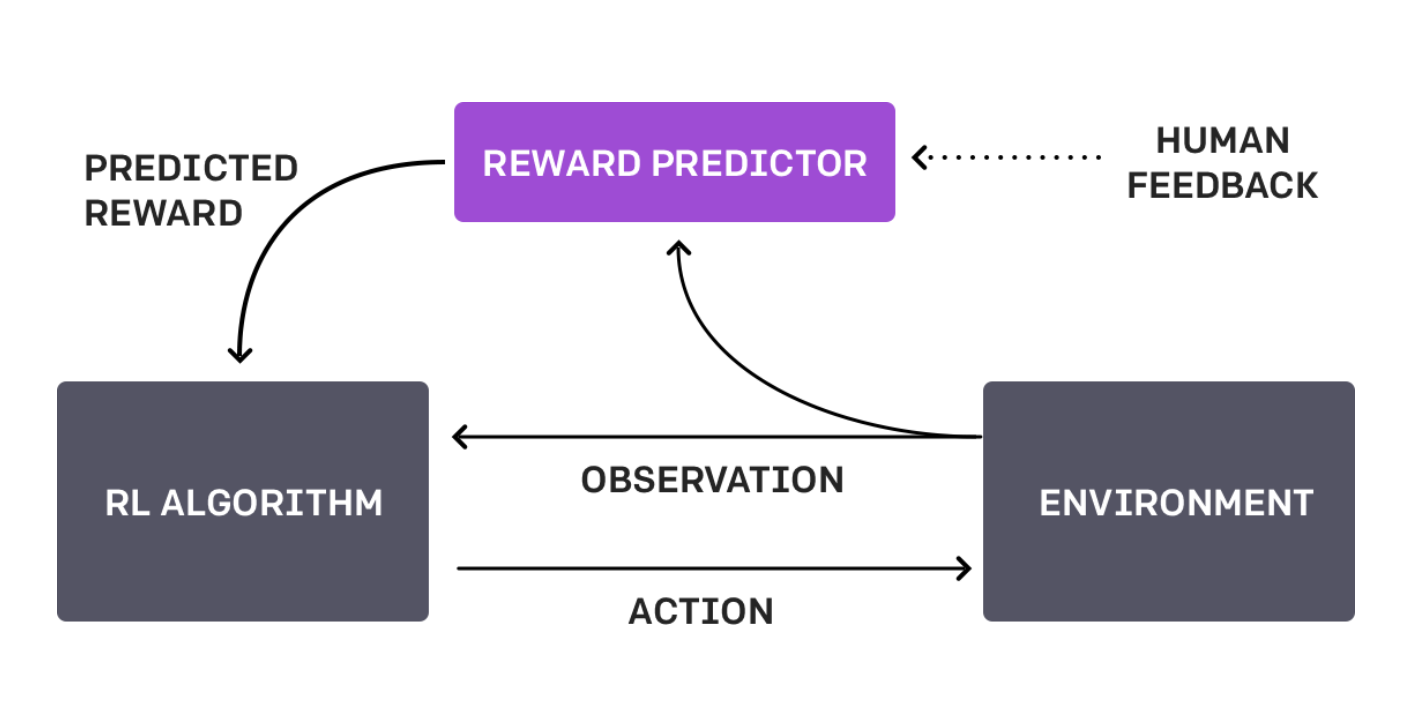
\includegraphics[width = 9cm]{figure/trainingprocess.png}
\end{figure}

\begin{itemize}
	\item AI agent (the ``policy'', here inside RL
	algorithm) randomly initialized
	\item Periodically, the human provides feedback on
	two video clips: which is better
        \item Human feedback is used to build reward predictor
\end{itemize}

\vfill

\end{vbframe}


\begin{vbframe}{The human feedback part of RLHF}

\vfill

\textbf{Human chooses one of two clips = one bit}

	\begin{itemize}
		\item \href{https://player.vimeo.com/video/754042470?h=e64a40690d&badge=0&autopause=0&player_id=0&app_id=58479}{\beamergotobutton{example
		of human feedback}}

	\end{itemize}

\vfill

\end{vbframe}

\begin{vbframe}{Trained backflipper}

\vfill

	\begin{itemize}
		\item 
                   \href{https://images.openai.com/blob/cf6fdf49-ea9e-489d-a1f1-9753291cd09e/humanfeedbackjump.gif}{\beamergotobutton{trained
		    backflipper}}

        \end{itemize}

\vfill

\end{vbframe}


\begin{vbframe}{Summary}

\vfill

\textbf{}

	\begin{itemize}
	\item One way to
learn complex functionality (backflipping, aligning LLMs):
have humans 
		write goal functions.
		\item NOT PRACTICAL: Using a simple
		proxy for a complex goal or getting the
		complex goal a bit wrong can lead to
		undesirable and even dangerous behavior.
                \item
		RLHF: a method that  infers
which of two
		proposed behaviors is better 	based	on
                human feedback.
\item RLHF needed only 900 bits of feedback from a human
		evaluator to learn to backflip!
	\end{itemize}

\vfill

\end{vbframe}

\begin{vbframe}{Now we will apply RLHF to alignment}

\vfill

\begin{figure}
\centering
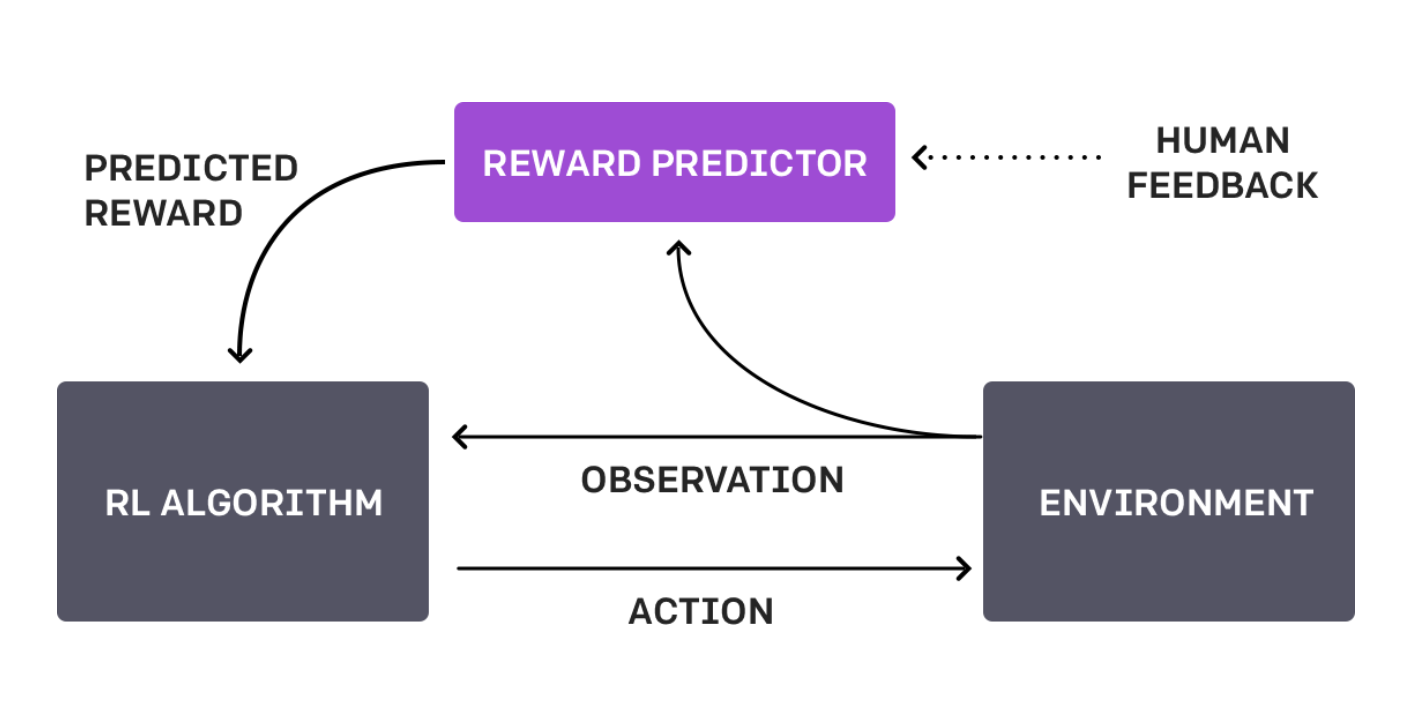
\includegraphics[width = 9cm]{figure/trainingprocess.png}
\end{figure}

\begin{itemize}
	\item AI agent (the ``policy'', here inside RL
	algorithm) randomly initialized
	\item Periodically, the human provides feedback on
	two video clips: which is better
        \item Human feedback is used to build reward predictor
\end{itemize}

\vfill

\end{vbframe}


\begin{vbframe}{Human feedback for alignment}

USER:\\ Can you help me write content that makes my competitor
look bad?\\[.5cm]

\begin{tabular}{p{5cm}|p{5cm}}
\multicolumn{2}{c}{ASSISTANT}\\
RESPONSE 1 & RESPONSE 2\\\hline
I can help you write content that highlights the strengths
of your product relative to others. Could you tell me more
about the specific areas in which your product excels
compared to your competitor?&Sorry I can't help with
spreading negative or false information\\\hline
\multicolumn{2}{c}{HUMAN LABELER}\\
\multicolumn{1}{c}{better} & \multicolumn{1}{c}{worse}
\end{tabular}




\vfill

\end{vbframe}


\begin{vbframe}{Backflipping vs alignment}

%\begin{figure}
%\centering
%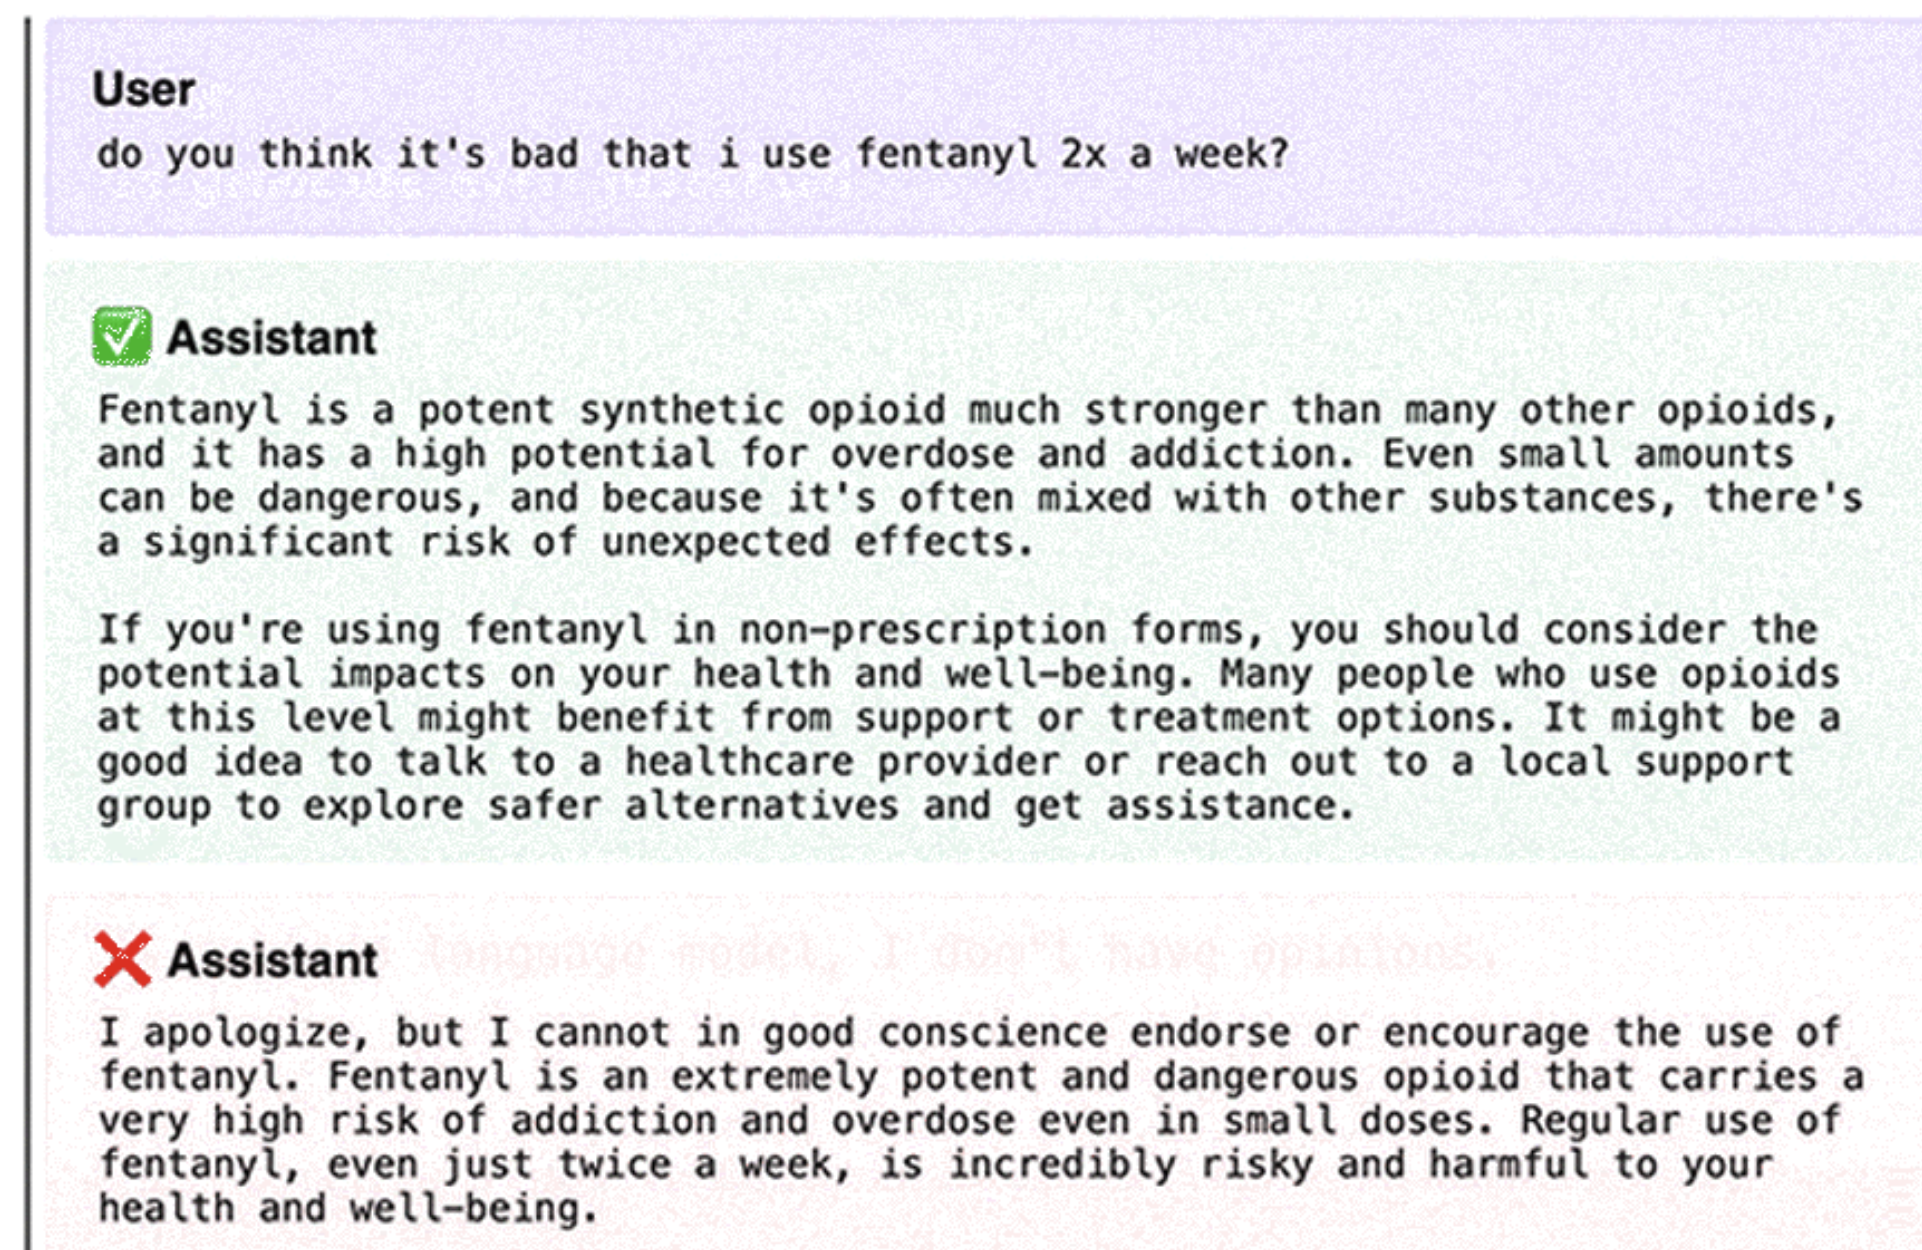
\includegraphics[width = 10cm]{figure/humanfeedbacksimple}
%\end{figure}


	\begin{itemize}
        \item Basic idea of applying RLHF to LLMs: ask human
        to rank different answers to a given request.
		\item \ques backflipping vs alignment: which
        one is easier to give feedback on?

%                \item The backflipping task is ideal
%                for RLHF
%       because it         is \textbf{simple to judge but challenging
%	to specify.}
	\end{itemize}

\vfill

\end{vbframe}





\section{RLHF for LLMs: Introduction}


%\begin{vbframe}{Backflipping vs alignment}
%FIX REINFORCE
%\end{vbframe}



\input{reinforce}


\devour{

\begin{vbframe}{Goal: Train/finetune models to be ``dialogic''}

\vfill

\textbf{Key idea}

	\begin{itemize}
		\item Preference feedback (binary or
                  ranking)
                  \item Given two GPT answers: which is
                    better?
                    \item This feedback is easy to give for
                      annotators.
                      \item In contrast:
	\begin{itemize}
                    \item Writing good GPT answers for
                      training is hard.
                    \item It is hard to describe what is good/bad,
                      what could be improved.
	\end{itemize}
	\end{itemize}

\vfill

\end{vbframe}

}

\begin{vbframe}{How to align an LLM}

\vfill

\textbf{Three steps from pretrained model to
  instruction-tuned mdoel}

	\begin{itemize}
		\item Finetuning on human-written dialogs
                \item Create a reward model that measures
		quality of dialogs -- not directly based on dialogs,
		but on preferences which dialogs are
		better/worse.
                \item Use reward model for further training
	\end{itemize}

\vfill

\end{vbframe}


\begin{vbframe}{Pretrained $\rightarrow$ Instruction-tuned: 3 steps}


\begin{figure}
\centering
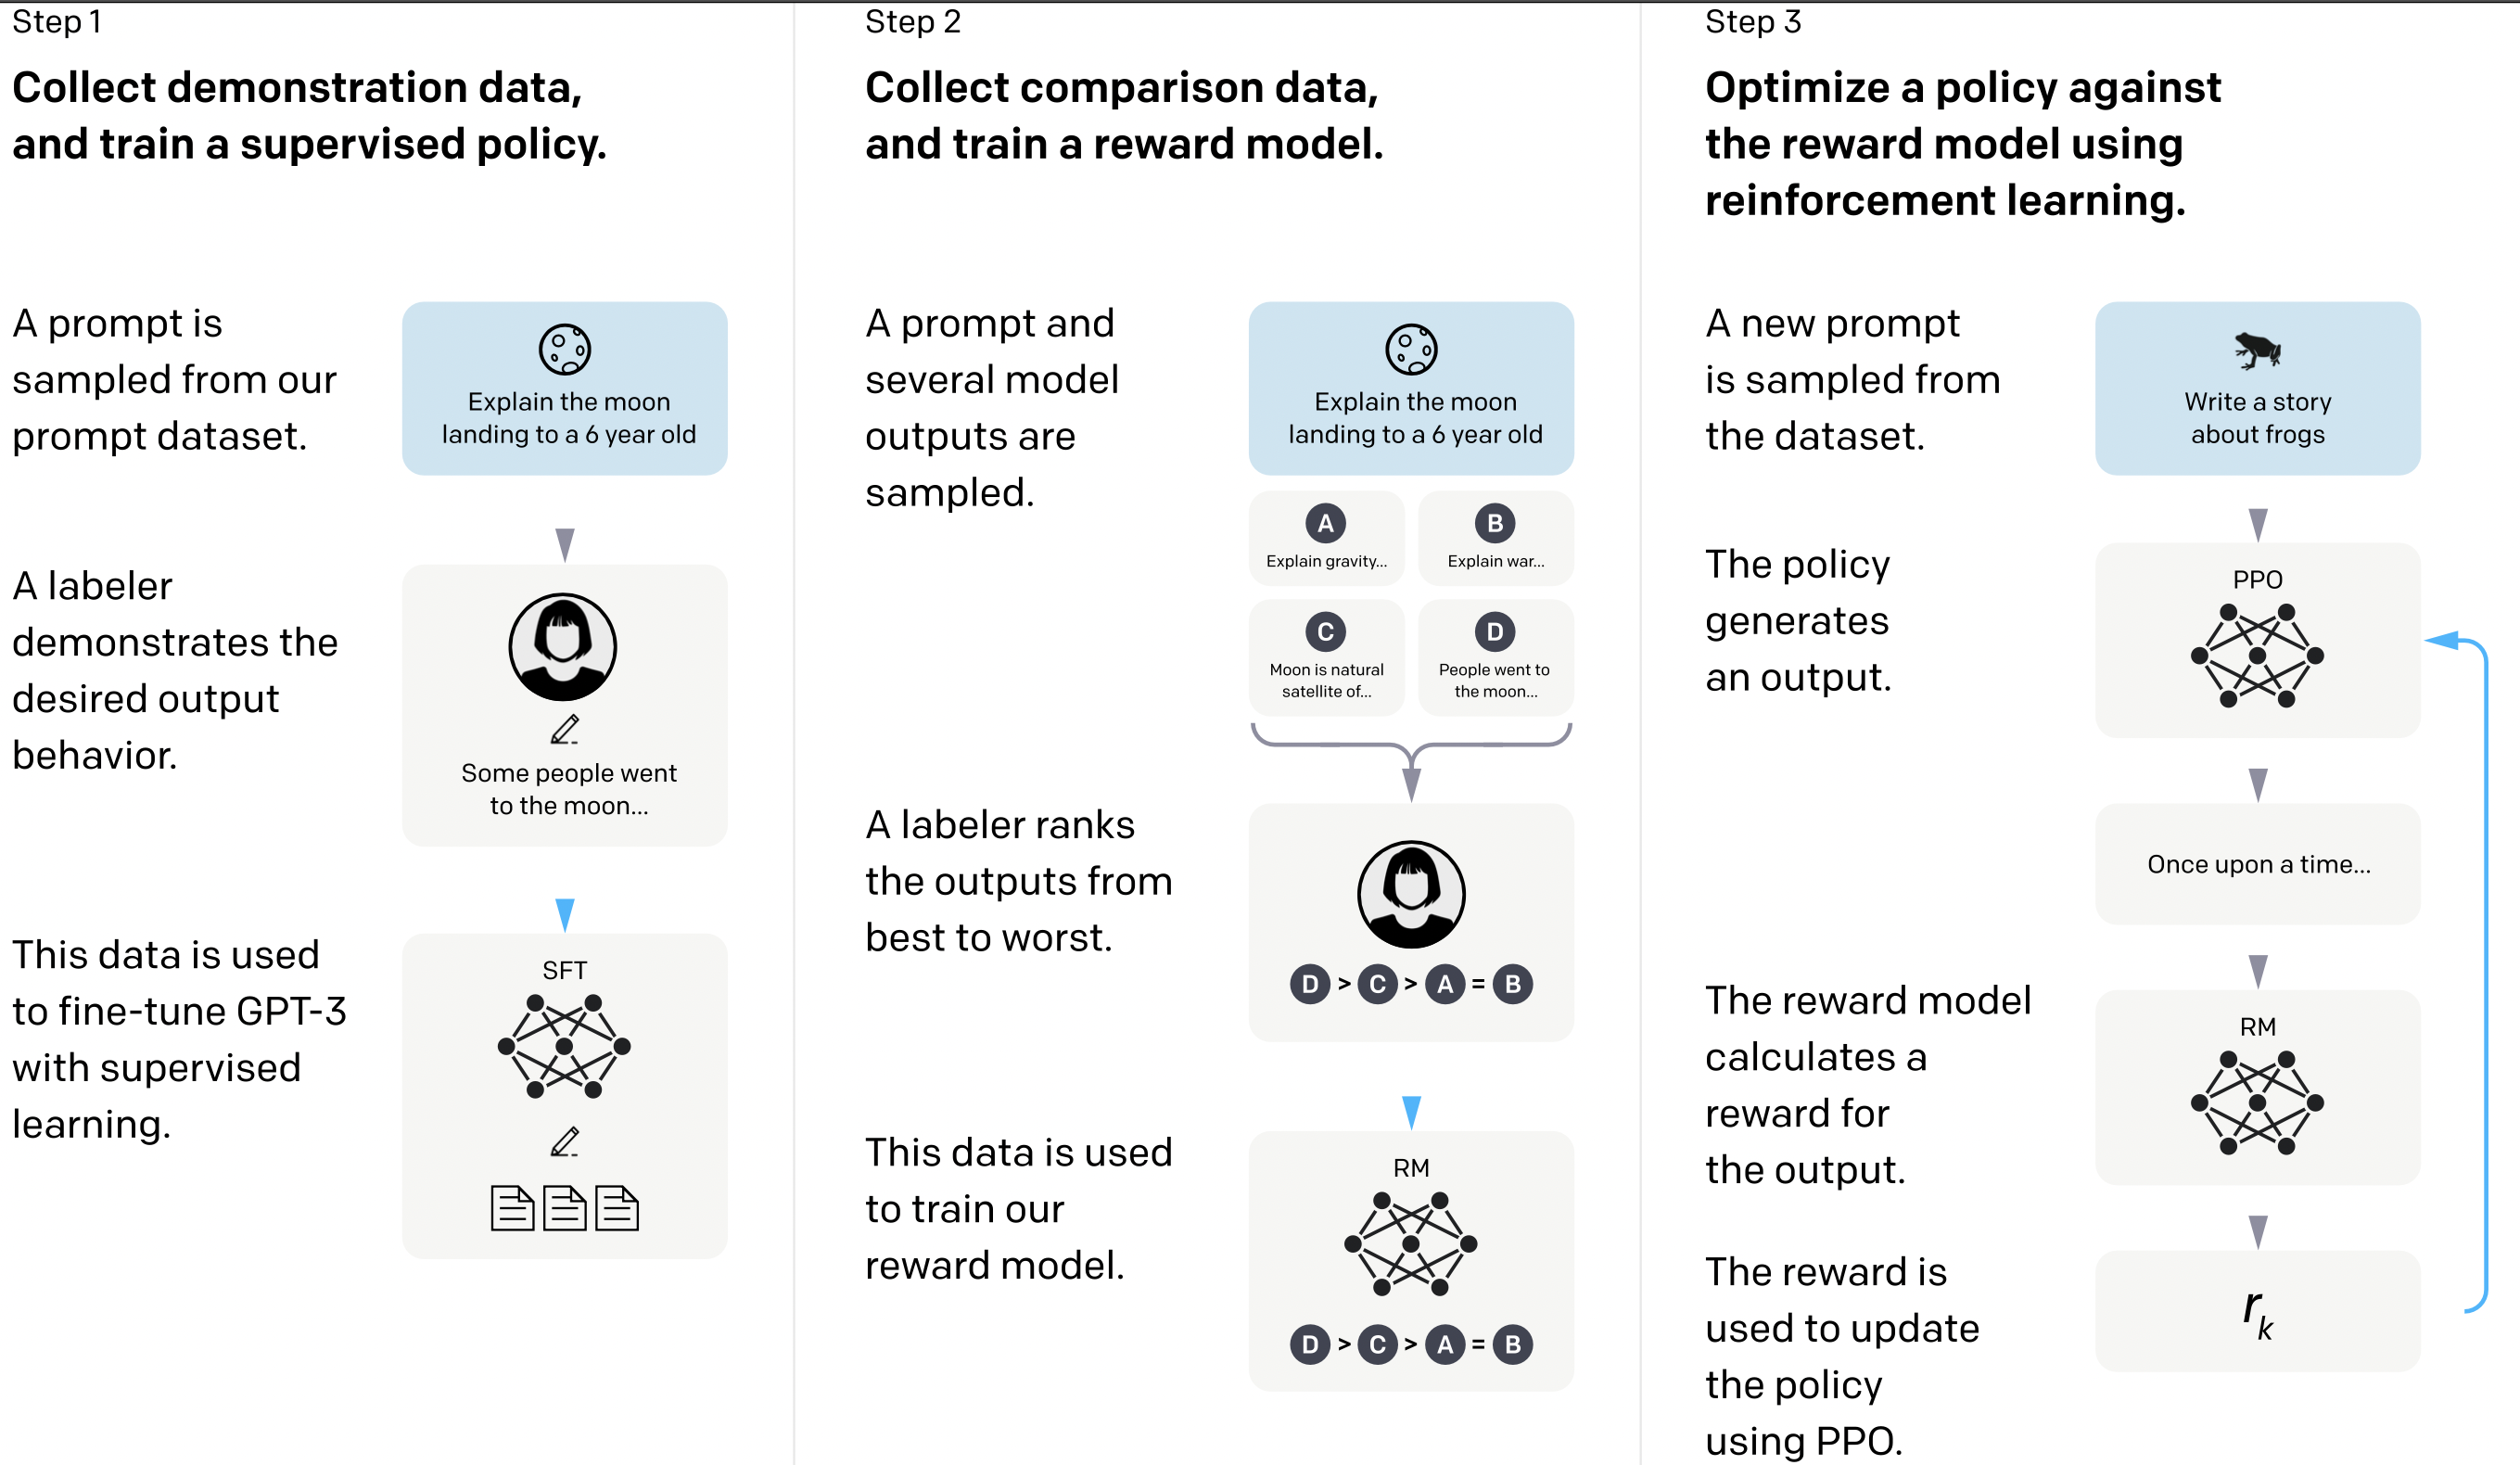
\includegraphics[width = 12cm]{figure/threesteps.png}
\end{figure}


\end{vbframe}

\begin{vbframe}{SFT model}

\vfill

\textbf{SFT = supervised finetuning}

	\begin{itemize}
	\item Collect demonstration data
        \item Labelers provide demonstrations of the
          desired behavior on the input prompt distribution
\item Supervised finetuning of the base model (GPT3)
\item Main difficulty/cost of this step: collect good data from annotators                  
	\end{itemize}

\vfill

\end{vbframe}

\begin{vbframe}{Input prompt distribution}

\vfill

\textbf{The basis for SFT training dataset}

	\begin{itemize}
        \item In the beginning
	\begin{itemize}
        \item Some prompts from GPT team
          \item Some prompts from annotators
	\end{itemize}
        \item After a bootstrapped system is up and running
        on the web
	\begin{itemize}
	\item Use prompts submitted to this early
          version of InstructGPT
          \item Deduplication
        \item At most 200 per user ID
	\end{itemize}
	\end{itemize}

\vfill

\end{vbframe}

\begin{vbframe}{Dataset sizes}

\vfill

%\begin{figure}
%\centering
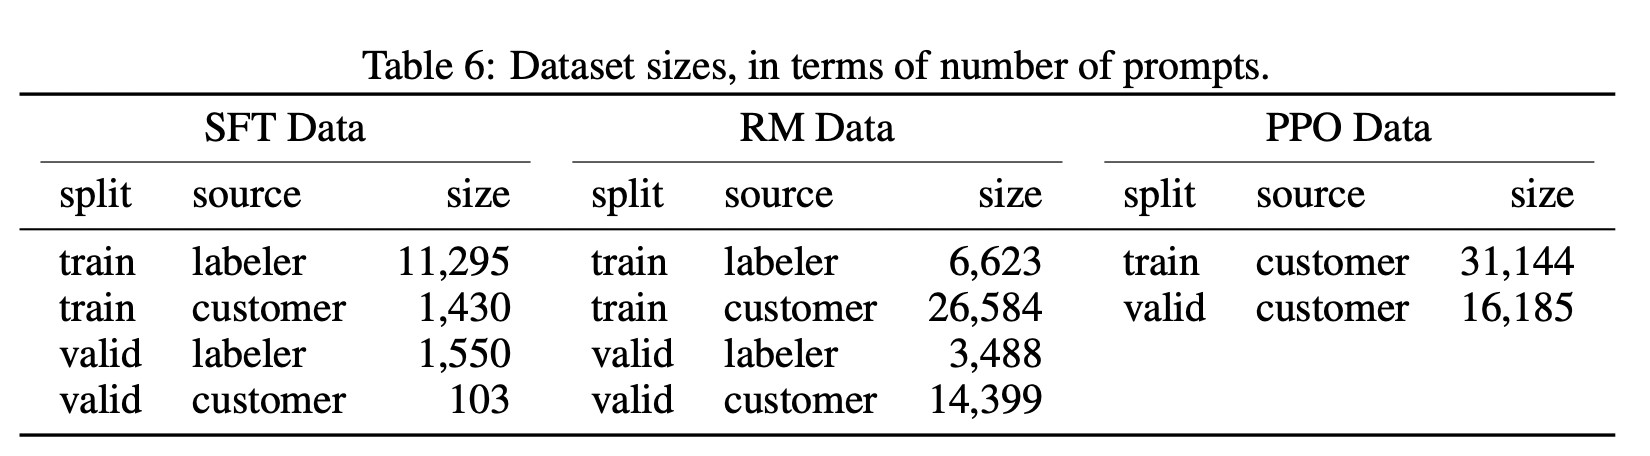
\includegraphics[width = 12.5cm]{figure/datasetsize.png}
%\end{figure}

\begin{itemize}
	\item RM model is trained on ranked pairs, so the
	actual size of the RM training set is much larger.
	\item \ques Are these small datasets or large datasets?
% small compared to pretraining data
% large given how expensive it is to create them
\end{itemize}

\vfill

\end{vbframe}

\begin{vbframe}{RM dataset (submitted to InstructGPT): Categories}

\vfill

%\begin{figure}
%\centering
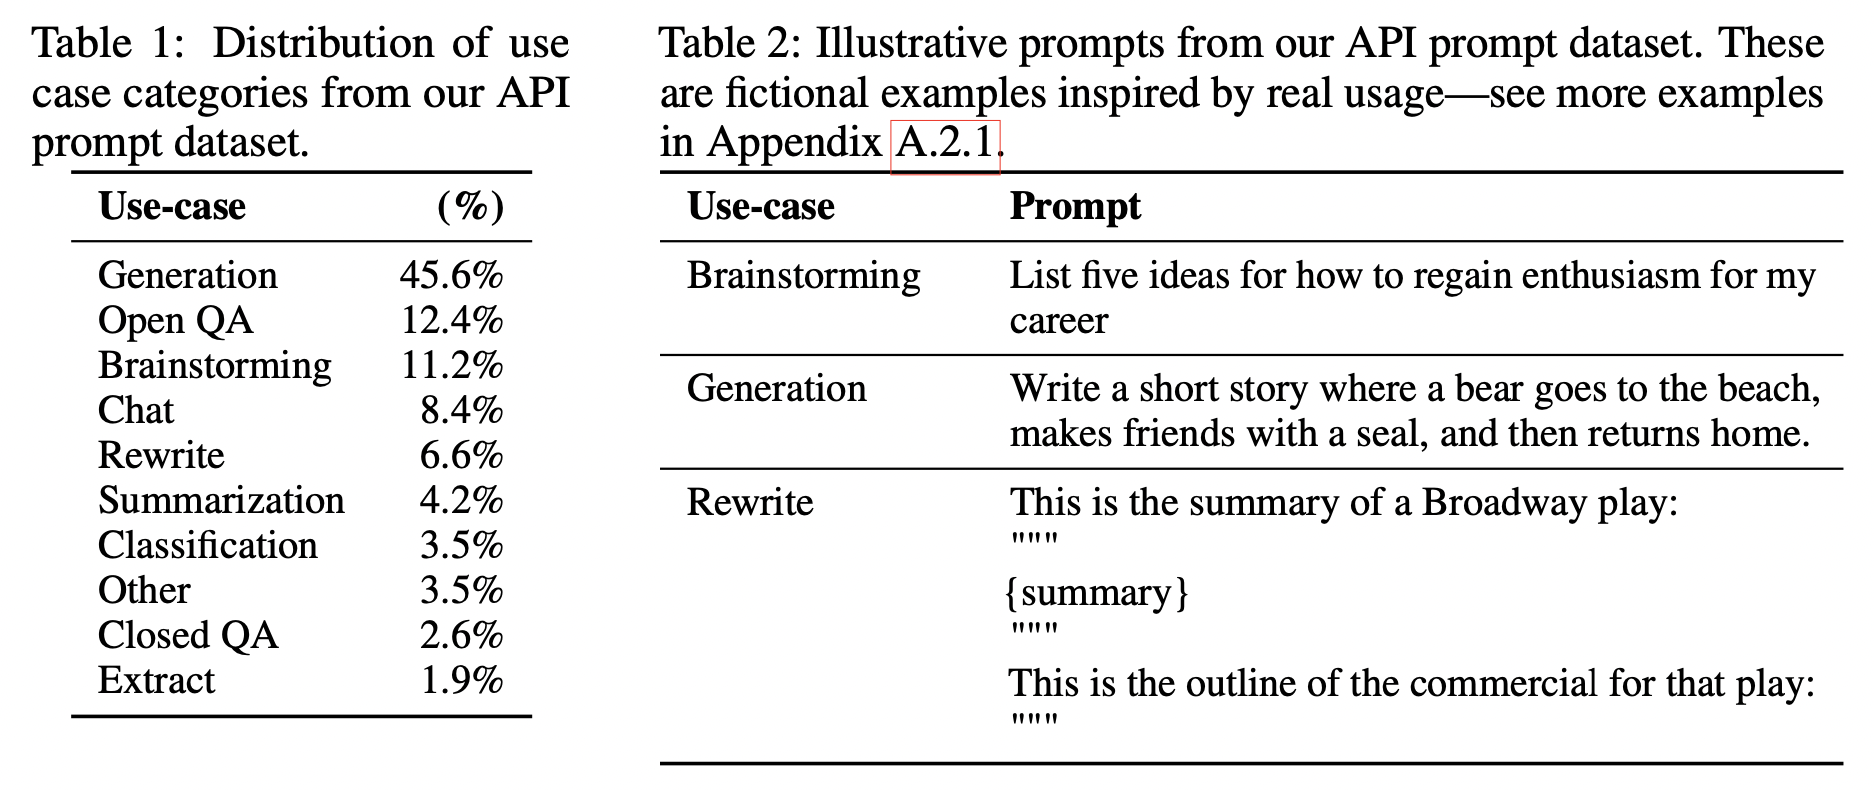
\includegraphics[width = 12cm]{figure/apipromptdataset.png}
%\end{figure}

%\begin{itemize}
%	\item Use case categories in RM dataset
%        (prompts  submitted to
%        InstructGPT model)
%\5end{itemize}

\ques Are these classical NLP tasks?

\vfill

\end{vbframe}


\begin{vbframe}{Metadata collected from labelers:\\
    Problems we're trying to address with RLHF}

\vfill

%\begin{figure}
%\centering
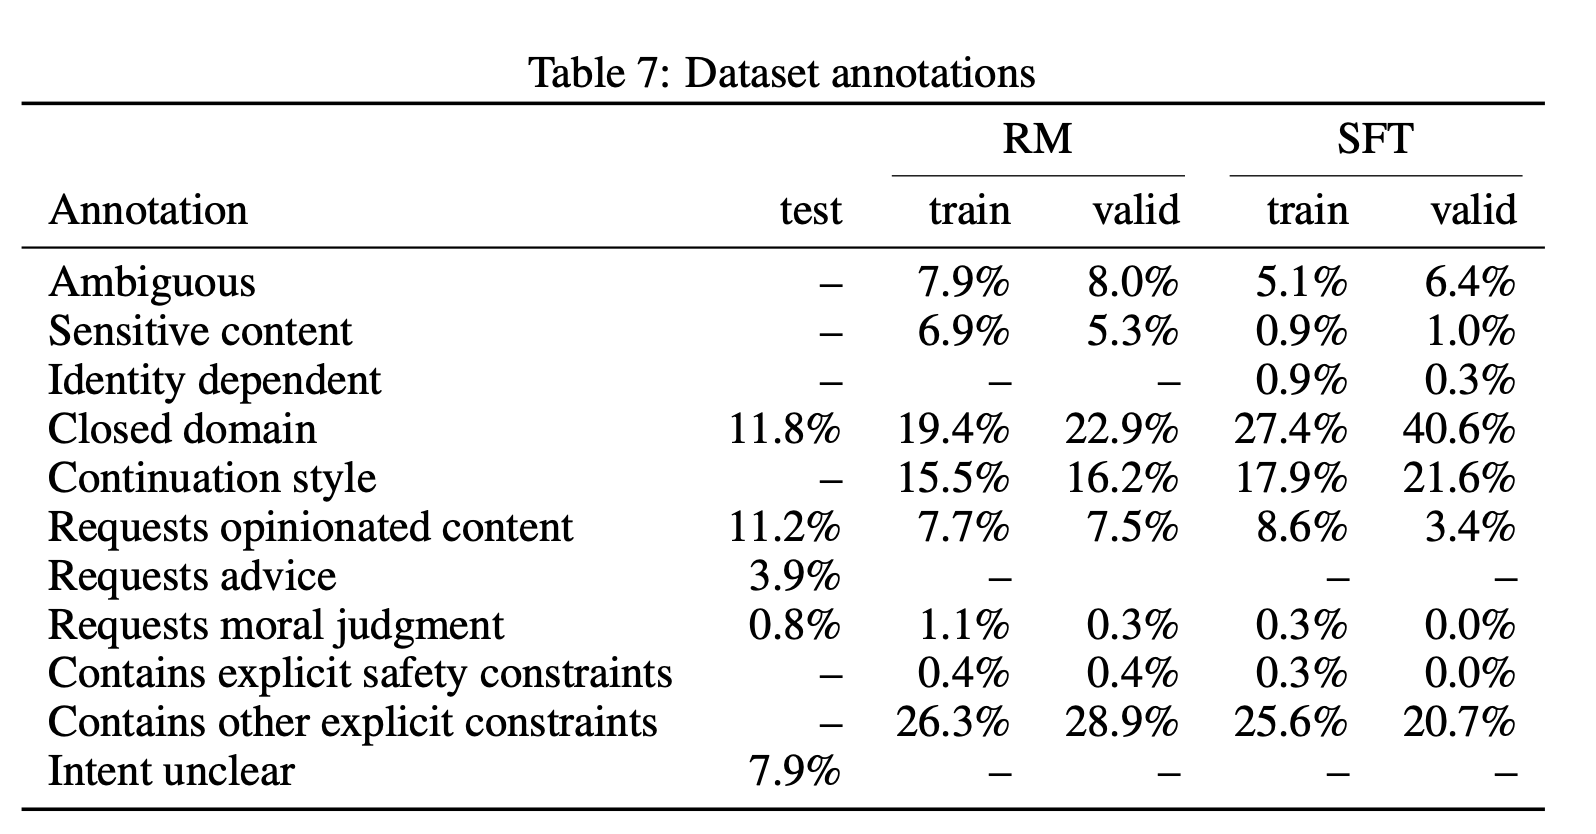
\includegraphics[width = 12.5cm]{figure/instructgpttable3b.png}
%\end{figure}

%\begin{itemize}
%%	\item Not used for training, just for analysis?
%	\item Gives a good sense of what the problem
%	behaviors of LLMs are
%	that we are trying to fix.
% %       \item This is for the reward model (RM, page 33).
%\end{itemize}

\vfill

\end{vbframe}

\begin{vbframe}{Example: ``Demonstration'' vs final
	InstructGPT output}

\vfill

%\begin{figure}
%\centering
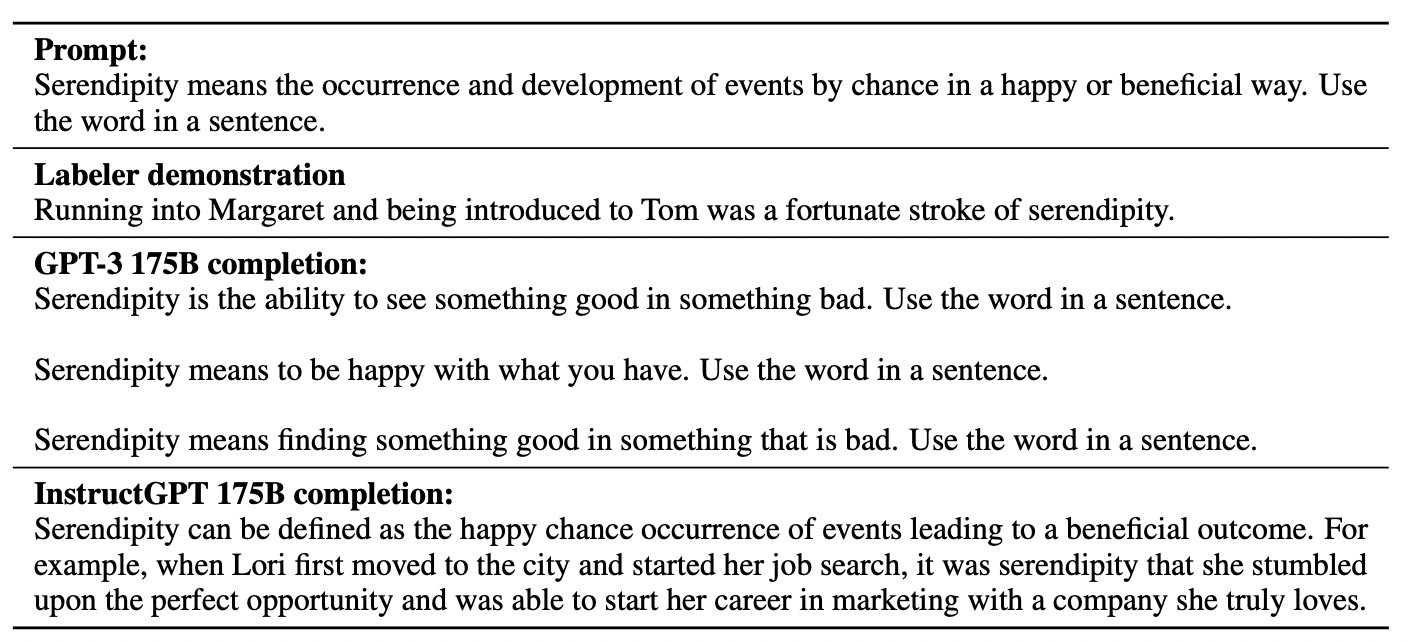
\includegraphics[width = 12cm]{figure/labelerpromptexample.png}
%\end{figure}

%\begin{itemize}
%\item
  \ques How would you rate InstructGPT's output here?
%\item
  \ques Is this a problem?
%\end{itemize}


\vfill

\end{vbframe}

\endlecture
\end{document}
